\documentclass[12pt]{article}
\newcommand{\template}{../../../template}
\usepackage{\template/packages}
\graphicspath{{assets/}}

\newcommand{\titolo}{Appunti di Intelligenza Artificiale}
\newcommand{\autore}{Rosso Carlo}
\newcommand{\data}{A.A. 2023/2024}
\newcommand{\corso}{Intelligenza Artificiale}

\newcommand{\copertina}{
	\begin{titlepage}
		\begin{center}
			\vspace*{3cm}
			\LARGE{\textbf{\titolo}}\\
			\vspace{0.33cm}
			\Large{\textbf{\data}}\\
			\vspace{0.33cm}
			\Large{\autore}\\
		\end{center}
		\thispagestyle{empty}
	\end{titlepage}
}


\begin{document}
\copertina
\tableofcontents
\newpage

\section{Introduzione}

\paragraph{Che cos'è l'intelligenza?}
La capacità di un agenti di affrontare e risolvere con successo situazioni e
problemi nuovi o sconosciuti.\\
I libri di testo classici definiscono l'IA come lo studio di agenti
intelligenti, che percepiscono il loro ambiente e producono azioni volte a
massimizzare la probabilità di successo nel raggiungere i loro scopi.

\paragraph{Intelligenza Artificiale stretta} si riferisce a qualsiasi
intelligenza artificiale in grado di eguagliare o superare un essere umano in un
compito strettamente definito e strutturato.

\paragraph{Intelligenza Artificiale generale} dovrebbe consentire alle macchine
di applicare conoscenze e abilità in diversi contesti anche di tipo nuovo. Si
tratta di un obiettivo non ancora realizzato e non è detto che sia possibile.\\

Lo scopo dell'IA può essere definito come quello di costruire "agenti
intelligenti". In particolare, l'IA studia come riprodurre in un computer 
processi mentali complessi. Questo conduce a due diverse prospettive:
\begin{itemize}
	\item construire dispositivi più intelligenti, che si avvicinano e superano
		l'intelligenza umana (prospettiva ingegneristica);

	\item costruire e testare ipotesi specifiche sui meccanismi all'interno 
		della scatola (cervello), per simulare e studiare il 
		comportamento umano anche quando questo non è ottimale (prospettiva 
		delle scienze congnitive).
\end{itemize}

\section{Fondamenti}

\subsection{Il neurone artificiale}

La descrizione degli elementi fondamentali dei circuiti neurali artificiali che
segue si riferisce a proprietà generali dei modelli presentati nei capitoli
successivi.\\
Un neurone artificiale è caratterizza da un insieme di sinapsi che corrispondono
ai terminali di altri neuroni, da una soglia e da una funzione di attivazione.
L'input netto o potenziale di attivazione $A_i$ di un neurone $i$ è la somma
algebrica dei prodotti fra tutti i segnali di ingresso $x_j$ e i valori dei pesi
corrispondenti $w_{ij}$:

\begin{equation*}
	A_i = \sum_{j=1}^{n} w_{ij}x_j
\end{equation*}

A cui solitamente si sottrae il valore di soglia $\theta_i$ del neurone:

\begin{equation*}
	A_i = \sum_{j=1}^{n} w_{ij}x_j - \theta_i
\end{equation*}

La risposta del neurone $y_i$ viene calcolata sottoponendo il potenziale di
attivazione ($A_i$) così ottenuto all'azione di una funzione di attivazione
$\phi(A)$:

\begin{equation*}
	y_i = \phi(A_i) = \phi(\sum_j^N w_{ij}x_j - \theta_i)
\end{equation*}

Nella maggior parte dei modelli il peso $w_{ij}$ può assumere valori positivi o
negativi continui (non interi, ovvero con la virgola) ed è il valore che si
modifica durante la fase di apprendimento.\\
Ora risulta vantaggioso analizzare il sistema in notazione vettoriale. Dato che
il potenziale di attivazione di un neurone è una funzione lineare di segnali di
ingresso, il potenziale di attivazione di un intero strato di neuroni $A^T = \{
	A_1, A_2, \ldots, A_n \}$ è riscrivibile come:

\begin{equation*}
	A = W \cdot x
\end{equation*}

Dove:
\begin{itemize}
	\item $x^T$ è il vettore dei segnali d'ingresso e possono essere sia valori
	      di input esterno (dall'ambiente) che valori di attivazione di uno
	      strato inferiore di unità;

	\item $W = \{w_{ij}\}$ è la matrice dei pesi sinaptici, con $w_{ij}$ che
	      rappresenta il peso della connessione tra l'unità $i$ e l'unità $j$;
\end{itemize}

\subsection{Rappresentazione}

Riporto alcune riflessioni sulle rappresentazione dei dati di input.\\
In generale le codifiche bipolari si rivelano vantaggiose rispetto alle
codifiche binarie. Infatti, permette di trattare dati incompleti in modo neutro,
al posto di usare $-1$ o $1$, il dato mancante può essere rappresentato con $0$,
che non ha alcun effetto sulle operazioni di somma e prodotto (quindi la
tangente iperbolica è una funzione di attivazione più adatta rispetto alla
sigmoide).\\

\subsubsection{Codifica locale}

Nella codifica locale, ogni unità di input rappresenta un determinato oggetto.
Si tratta di una rappresentazione molto semplice, ma ha diversi svantaggi:
\begin{enumerate}
	\item richiede un alto numero di unità di input: ovvero $n$ unità per
	      rappresentare $n$ oggetti;

	\item richiede di conoscere il numero di oggetti da rappresentare in
	      anticipo;

	\item è molto fragile alla perdita di un'unità di input, che corrisponde
	      alla perdita dell'oggetto che rappresenta.
\end{enumerate}

\subsubsection{Codifica distribuita}

Nella codifica distribuita, gli oggetti sono rappresentati da un codice binario
di $n$ nodi che rappresentano $2^n$ oggetti. Anche questa rappresentazione ha
alcuni svantaggi:
\begin{enumerate}
	\item mancanza di flessibilità: non è possibile rappresentare nuovi oggetti
	      senza modificare la struttura della rete;

	\item fragilità: la perdita di un nodo di input può portare alla perdita
	      di un'informazione significativa.
\end{enumerate}

\subsubsection{Codifica grezza}

Una soluzione proposta codifica le caratteristiche degli oggetti. Per cui
ciascun oggetto è descrivibile da un insieme di caratteristiche (e.g. peso,
colore, altezza, ecc.). Ciascuna unità di input codifica la presenza o il valore
di una certa caratteristica. Questa rappresentazione ha diversi vantaggi:

\begin{enumerate}
	\item flessibilità: è possibile rappresentare nuovi oggetti senza modificare
	      la struttura della rete;

	\item robustezza: la perdita di un'unità di input, comporta la perdita di
	      una caratteristica dell'oggetto, ma sono comunque presenti altre
	      caratteristiche che permettono di identificare l'oggetto.
\end{enumerate}

Le unità di input possono essere rappresentate come uno spazio
multi-dimensionale con tante dimensioni quante sono le unità. Oggetti con
caratteristiche simili saranno rappresentati da punti vicini nello spazio
multi-dimensionale. Per cui questa codifica facilita la classificazione e
generalizzazione della rete neurale.

\subsubsection{Campi recettivi sovrapposti}

C'è un altro modo per ottenere una codifica grezza: si tassella l'input (e.g.
l'immagine) in zone di dimensioni uguali e parzialmente sovrapposte. In questo
caso, l'accuratezza della rappresentazione dipende dalla dimensione delle zone e
dal numero di zone che coprono l'input. Approfondiamo le implicazioni che hanno
le dimensioni e il numero di zone sulle informazioni che possono essere
estratte:
\begin{itemize}
	\item \textbf{campi recettivi piccoli e non sovrapposti}: sono usate per
	      categorizzare le figure;

	\item \textbf{campi recettivi grandi e parzialmente sovrapposti}: sono usate
	      per distinguere le singole figure. Infatti, larghi campi recettivi
	      fanno sì che piccole caratteristiche possano essere codificate su un
	      numero maggiore di nodi, permettendo una maggior discriminazione dei
	      dettagli.
\end{itemize}

\subsubsection{Preparazione}

Prendendo spunto dalla biologia, risulta utile preparare i dati prima di essere
dati in pasto alla rete neurale. Per esempio, si possono filtrare i dati, oppure
si esegue la derivata sulle immagini per evidenziare i bordi e annullare i
colori, senza perdere informazioni utili allo scopo del modello.\\
In alternativa, si può usare una cascata di nodi con campi recettivi localmente
ristretti in modo che l'ampiezza della finestra attraverso la quale ogni nodo
osserva l'immagine diventa più grande man mano che si procede verso strati di
elaborazione sucessiva.

\subsubsection{Normalizzazione}

Un'altra operazione che può essere eseguita sui dati è la normalizzazione.
Questa operazione è utile per rendere i dati indipendenti dalla scala:

\begin{equation*}
	x' = \frac{x}{||x||} = \frac{x}{\sqrt{\sum_{i=1}^{n} x_i^2}}
\end{equation*}

In questo modo la lunghezza del vettore ottenuto sarà sempre 1.

\begin{center}
	\begin{tikzpicture}[scale=1.5]
		% Asse x
		\draw[->] (0,0) -- (2,0) node[right] {{}};
		\draw (1,0.1) -- (1,-0.1) node[below] {{1}};

		% Asse y
		\draw[->] (0,0) -- (0,2) node[above] {{}};
		\draw (0.1,1) -- (-0.1,1) node[left] {1};

		\draw[dashed, black] (0,0) -- (1,0) arc (0:90:1) -- cycle;
		\filldraw[black] (1.5,0.5) circle (1pt) node[right] {$x_1$};
		\filldraw[black] (0.2,0.7) circle (1pt) node[right] {$x_2$};

		\draw[black, fill=white] (0.949,0.316) circle (1pt) node[right] {$x_1'$};
		\draw[black, fill=white] (0.275,0.962) circle (1pt) node[right] {$x_2'$};
	\end{tikzpicture}
\end{center}

\subsection{Apprendimento}

La risposta di una rete neurale è determinata dai valori sinaptici delle
connessioni fra i nodi. Le reti neurali artificiali apprendono modificando
gradulamente i propri valori sinaptici attraverso la presentazione ripetuta di
una serie di esempi. Si distinguono tre tipi di apprendimento:
\begin{itemize}
	\item \textbf{Apprendimento supervisionato}: la modifica dei valori
	      sinaptici avviene impiegando una misura di errore tra la risposta
	      fornita dalla rete neurale e la risposta desiderata per ogni vettore
	      di input;

	\item \textbf{Apprendimento per rinforzo}: L'apprendimento supervisionato
	      include anche una gamma di algoritmi che richiedono solamente una
	      misura di bontà della risposta della rete neurale, piuttosto che la
	      specificazione della risposta esatta per ogni pattern di input. Questi
	      algoritmi sono denominati algoritmi di apprendimento per rinforzo;

	\item \textbf{Apprendimento non supervisionato}: sono anche chiamati
	      apprendimento per auto-organizzazione. In questo caso, la rete
	      neurale deve apprendere a riconoscere regolarità nei dati di input, in
	      quanto la risosta desiderata è sconosciuta e deve essere individuata
	      dalla rete medesima. Molti algoritmi di apprendimento senza
	      supervisore derivano da una precisa formulazione dell'informazione che
	      deve essere estratta dall'ambiente e richiedono dettagliate assunzioni
	      sulla struttura dei pattern di input.
\end{itemize}

Approfondiamo ora le caratteristiche comuni a tutti i tipi di apprendimento:
\begin{enumerate}
	\item \textbf{Stato iniziale}: i pesi iniziali sono assegnati in modo
	      casuale entro un piccolo campo di variazione (e.g. $[-0.1, 0.1]$),
	      oppure sono messi a zero;

	\item \textbf{Iterazione}: l'apprendimento consiste nella presentazione
	      ripetuta di una serie di vettori, detti anche pattern d'addestramento;

	\item \textbf{Nuove conoscenze}: Gli algoritmi di apprendimento
	      riguardano il calcolo di $\Delta w_{ij}$, la modifica dei pesi
	      rispetto al valore corrente:

	      \begin{equation*}
		      w_{ij}^t = w_{ij}^{t-1} + \Delta w_{ij}^{t}
	      \end{equation*}

	\item \textbf{Tasso di apprendimento}: la velocità di apprendimento è
	      regolata da una costante $\eta$:

	      \begin{equation*}
		      w_{ij}^t = w_{ij}^{t-1} + \eta \Delta w_{ij}^{t}, \quad 0 < \eta < 1
	      \end{equation*}

	\item \textbf{Test}: quando l'apprendimento è completato, i pesi sono
	      "congelati" e si studia la risposta della rete neurale su dei pattern
	      di test, che non sono stati usati durante l'apprendimento. Questo non
	      è vero per gli algoritmi che operano all'interno della Teoria della
	      Risonanza Adattiva.
\end{enumerate}

\subsection{Analisi vettoriale di un neurone artificiale}

Per semplificare l'analisi consideriamo il caso di un singolo neurone $i$, tale
che:
\begin{equation*}
	n_i = \phi(\sum_{j=1}^{n} w_{ij}x_j - \theta_i) = w \cdot x
\end{equation*}

La risposta dell'unità $n_i$ è una misura della somiglianza tra il vettore di
input ed il peso sinaptico. Come abbiamo già visto la norma (o lunghezza) di un
vettore $x$ è definita come:
\begin{equation*}
	||x|| = \sqrt{\sum_{j=1}^{n} x_j^2}
\end{equation*}

Il coseno dell'angolo $\theta$ tra due vettori $x$ e $w$ è definito come:
\begin{equation*}
	\cos(\theta) = \frac{w \cdot x}{||w|| \cdot ||x||}, 0 \leq \theta \leq \pi
\end{equation*}

Quindi, il prodotto interno $n_i = w \cdot x$ è
\begin{equation*}
	n_i = ||w|| \cdot ||x|| \cdot \cos(\theta)
\end{equation*}

Questo significa che muovendo nello spazio i due vettori mantenendo costante la
loro lunghezza, il loro prodotto interno sarà proporzionale al coseno
dell'angolo $\theta$ tra i due vettori. Ovvero, minore è l'angolo e maggiore è
il prodotto interno. In particolare il prodotto interno sarà massimo quando i
due vettori sono allineati, vale 0 quando sono ortogonali e sarà minimo quando
sono opposti (e $\max = -\min$, al variare dell'angolo).\\
Infine, è importante notare che in una rete neurale è possibile giudicare quale
unità possieda il vettore sinaptico più simile al vettore di input solo se i
vettori sinaptici sono normalizzati.

\subsection{Apprendimento hebbiano}

La regola di modifica sinaptica di Hebb costituisce le fondamenta su cui si
basano o derivano tutti gli algoritmi di apprendimento. Approfondiamo l'uso
delle regole hebbiane in una rete etero-associativa feedforward con un singolo
strato di snapsi e con unità binarie. Consideriamo un algoritmo di apprendimento
supervisionato.

\begin{figure}[H]
	\centering
	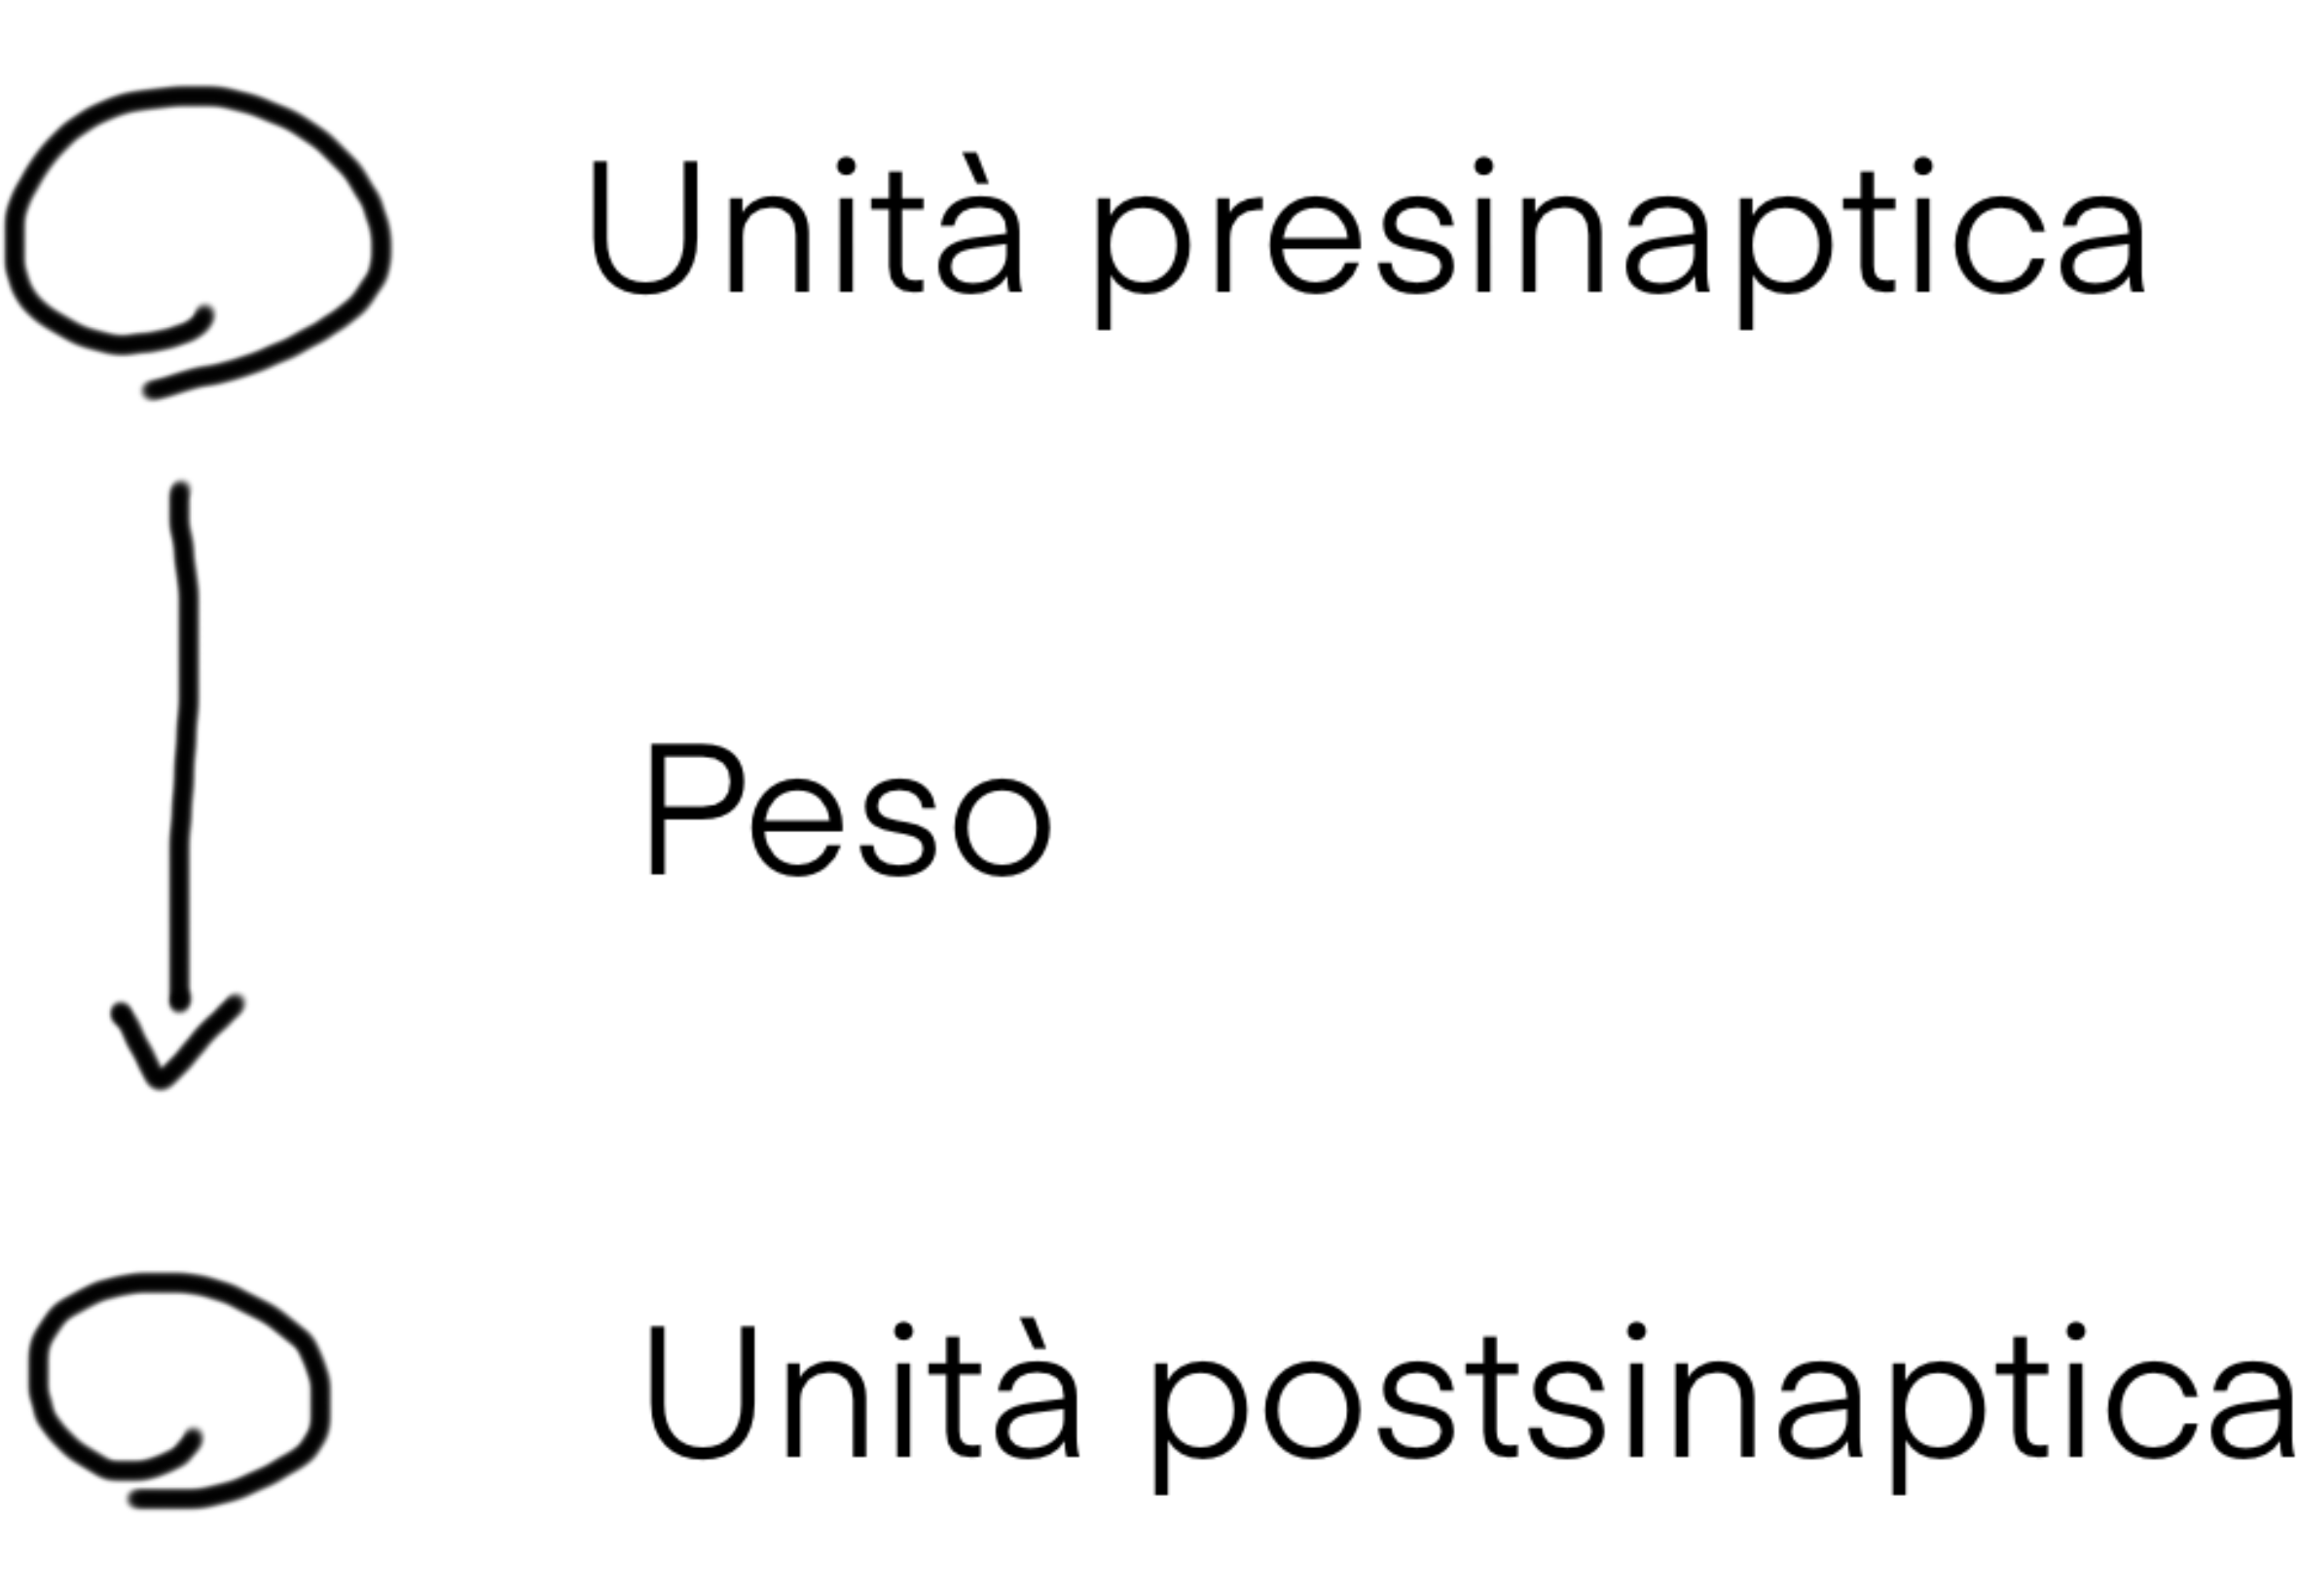
\includegraphics[width=0.3\textwidth]{Hebb}
	\caption{Rete neurale etero-associativa feedforward con un singolo strato di
		sinapsi e con unità binarie.}
\end{figure}

\subsubsection{La regola di Hebb}

Se due neuroni collegati tra di loro sono contemporaneamente attivi, il loro
peso viene incrementato. La regola di Hebb prevede solamente l'incremento dei
pesi, per cui la rete non è in grado di apprendere associazioni che presentano
elementi in comune, ma che richiedono risposte differenti. Dunque la regola di
Hebb permette di apprendere solamente pattern di input che sono ortogonali tra
loro.

\subsubsection{La regola postsinaptica}

Questa regola è anche chiamata regola di Stent-Singer. Il peso viene
incrementato ogni volta che l'unità postsinaptica e l'unità presinaptica sono
entrambe attive; inoltre viene diminuito ogni volta che l'unità postsinaptica è
attiva, ma quella presinaptica è inattiva. Questa regola migliora la generalità,
tuttavia, non fallisce l'apprendimento di pattern di input parzialmente
sovrapposti sullo stesso output, perché tende a creare troppe sinapsi
inibitorie.

\subsubsection{La regola presinaptica}

Il peso viene aumentato quando sia l'unità presinaptica che l'unità
postsinaptica sono attive; il peso viene diminuito quando l'unità presinaptica è
attiva, ma l'unità postsinaptica è inattiva. Questa regola permette di
generalizzare molto meglio rispetto alle regole precedenti.

\subsubsection{La regola della covarianza}

Viene anche chiamata regola di Hopfield. Quando l'unità presinaptica e l'unità
postsinaptica hanno lo stesso stato, il peso viene incrementato; quando hanno
stati opposti, il peso viene diminuito.

\begin{table}[H]
	\centering
	\begin{tabular}{lcccc}
		\hline
		Unità presinaptica  & + & +   & $-$ & $-$ \\
		Unità postsinaptica & + & $-$ & +   & $-$ \\
		\hline
		Hebb                & + &     &     &     \\
		Postsinaptica       & + &     & $-$ &     \\
		Presinaptica        & + & $-$ &     &     \\
		Covarianza          & + & $-$ & $-$ & +   \\
		\hline
	\end{tabular}
	\caption{Riassunto del funzionamento delle regole hebbiane.}
\end{table}

Concludendo, le regole di Hebb possiedono parecchie limitazioni nel tipo di
associazioni che sono in grado di apprendere, poiché sono spesso soggette a
fenomeni di interferenza quando gli input d'ingresso non sono linearmente
indipendenti.

\section{Regola Delta}

La regola delta è applicabile a unità di output dotate di una funzione di
attivazione continua e differenziabile. Questa caratteristica permette di
descrivere le prestazioni di una rete neurale tramite una funzione continua
$E_w$ che misura l'errore della rete.

\subsection{Unità lineari}

Consideriamo una rete neurale di tipo feedforward con unità di output ad
attivazione lineare:

\begin{equation}
	y_i = \sum_{j=1}^n w_j x_j
\end{equation}

L'obiettivo è ottenere una matrice di pesi sinaptici $W$, per cui ogni esempio
restituisce in output il valore corretto, ovvero ciascun esempio viene
classificato correttamente:

\begin{equation*}
	y^{\mu}_i = t^{\mu}_i \quad \forall i, \mu
\end{equation*}


dove $t^{\mu}_i$ è l'output corretto ($t$ sta per \textit{target}) per l'input $\mu$-esimo sul neurone
$i$-esimo. La funzione di errore è definita come:

\begin{equation}
	E_W = \frac{1}{2} \sum_{\mu} \sum_{i} (t^{\mu}_i - y^{\mu}_i)^2
\end{equation}

Ovvero, viene calcolata la distanza (lo scarto quadratico medio) tra l'output
desiderato e quello effettivo
per ogni esempio e per ogni neurone di output. L'obiettivo è minimizzare la
funzione di errore $E$, infatti nel caso in cui tutti gli esempi vengano
classificati correttamente, l'errore sarà nullo ($E_W = 0$).
Dunque dobbiamo capire in quale direzione muovere i pesi per ridurre l'errore.
La derivata della funzione di errore rispetto ai pesi ci fornisce la pendenza
del grafico, ovvero dato un punto dello spazio dei pesi (individuato dai pesi
sinaptici correnti) ci indica quali pesi aumentare e quali diminuire per ridurre
il valore dell'errore. In particolare:

\begin{equation}
	\Delta w_{ij} = - \frac{\partial E_W}{\partial w_{ij}}
\end{equation}

ci indica in quale direzione muovere il peso $w_{ij}$ per ridurre l'errore,
indica a tutti gli effetti la pendenza del grafico dell'errore rispetto al peso
e quindi in quale direzione si muove una pallina che rotola lungo il grafico.
Calcoliamo dunque le derivate che ci interessano:

\begin{equation}
	\Delta w_{ij} = \sum_{\mu}(t^{\mu}_i - y^{\mu}_i) x^{\mu}_j
\end{equation}

Interpretiamo la formula: per ciascun esempio $\mu$ calcoliamo la differenza tra
il valore desiderato e quello effettivo, moltiplichiamo il risultato per il
valore dell'input $j$-esimo e sommiamo il tutto per ciascun esempio. Notiamo che
se ci fosse solo un esempio, dopo il cambio di peso l'errore sarebbe nullo,
infatti si va a modificare il peso in modo tale che l'output sia uguale al
target. Sommando le variazioni per ogni esempio, si ottiene la variazione totale
dei pesi, per avvicinare l'output effettivo a quello desiderato, non è detto che
esso sia raggiunto, ma ci si avvicina.

\subsection{Unità non lineari}

Allo stesso modo possiamo calcolare la variazione dei pesi per unità di output
dotate di una funzione di attivazione non lineare. In particolare, data una
funzione di attivazione $\phi$ e un output $y_i$ calcolato come:

\begin{equation}
	y_i = \phi(\sum_{j=1}^n w_{ij} x_j)
\end{equation}

La variazione dei pesi è calcolata come:

\begin{equation}
	\Delta w_{ij} = \sum_{\mu}(t^{\mu}_i - y^{\mu}_i) \phi'(\sum_j w_{ij} x^\mu_j) x^{\mu}_j
\end{equation}

Dove $\phi'(\sum_j w_{ij} x^\mu_j)$ è la derivata della funzione di attivazione
rispetto all'input. Poiché la formula diventa lunga e complessa,
poniamo $A^{\mu}_i = \sum_j w_{ij} x^\mu_j$, per cui
$y^{\mu}_i = \phi(A^{\mu}_i)$, ottenendo:

\begin{equation}
	\Delta w_{ij} = \sum_{\mu}(t^{\mu}_i - y^{\mu}_i) \phi'(A^{\mu}_i) x^{\mu}_j
\end{equation}

Dunque per ogni esempio $\mu$ la modifica dei pesi sinaptici diventa:

\begin{equation}
	\Delta w_{ij} = \eta (t_i - y_i) \phi'(A_i) x_j
\end{equation}

\section{Back-propagation}

Il metodo di propagazione all'indietro dell'errore è applicabile a reti neurali
con un numero qualsiasi di strati di connessioni e con architetture molto
diverse. Proprio come la regola delta, modifica i pesi sinaptici in base alla
discrepanza tra la risposta fornita dalla rete e la risposta corretta.

\subsection{Algoritmo}

\begin{figure}[H]
	\centering
	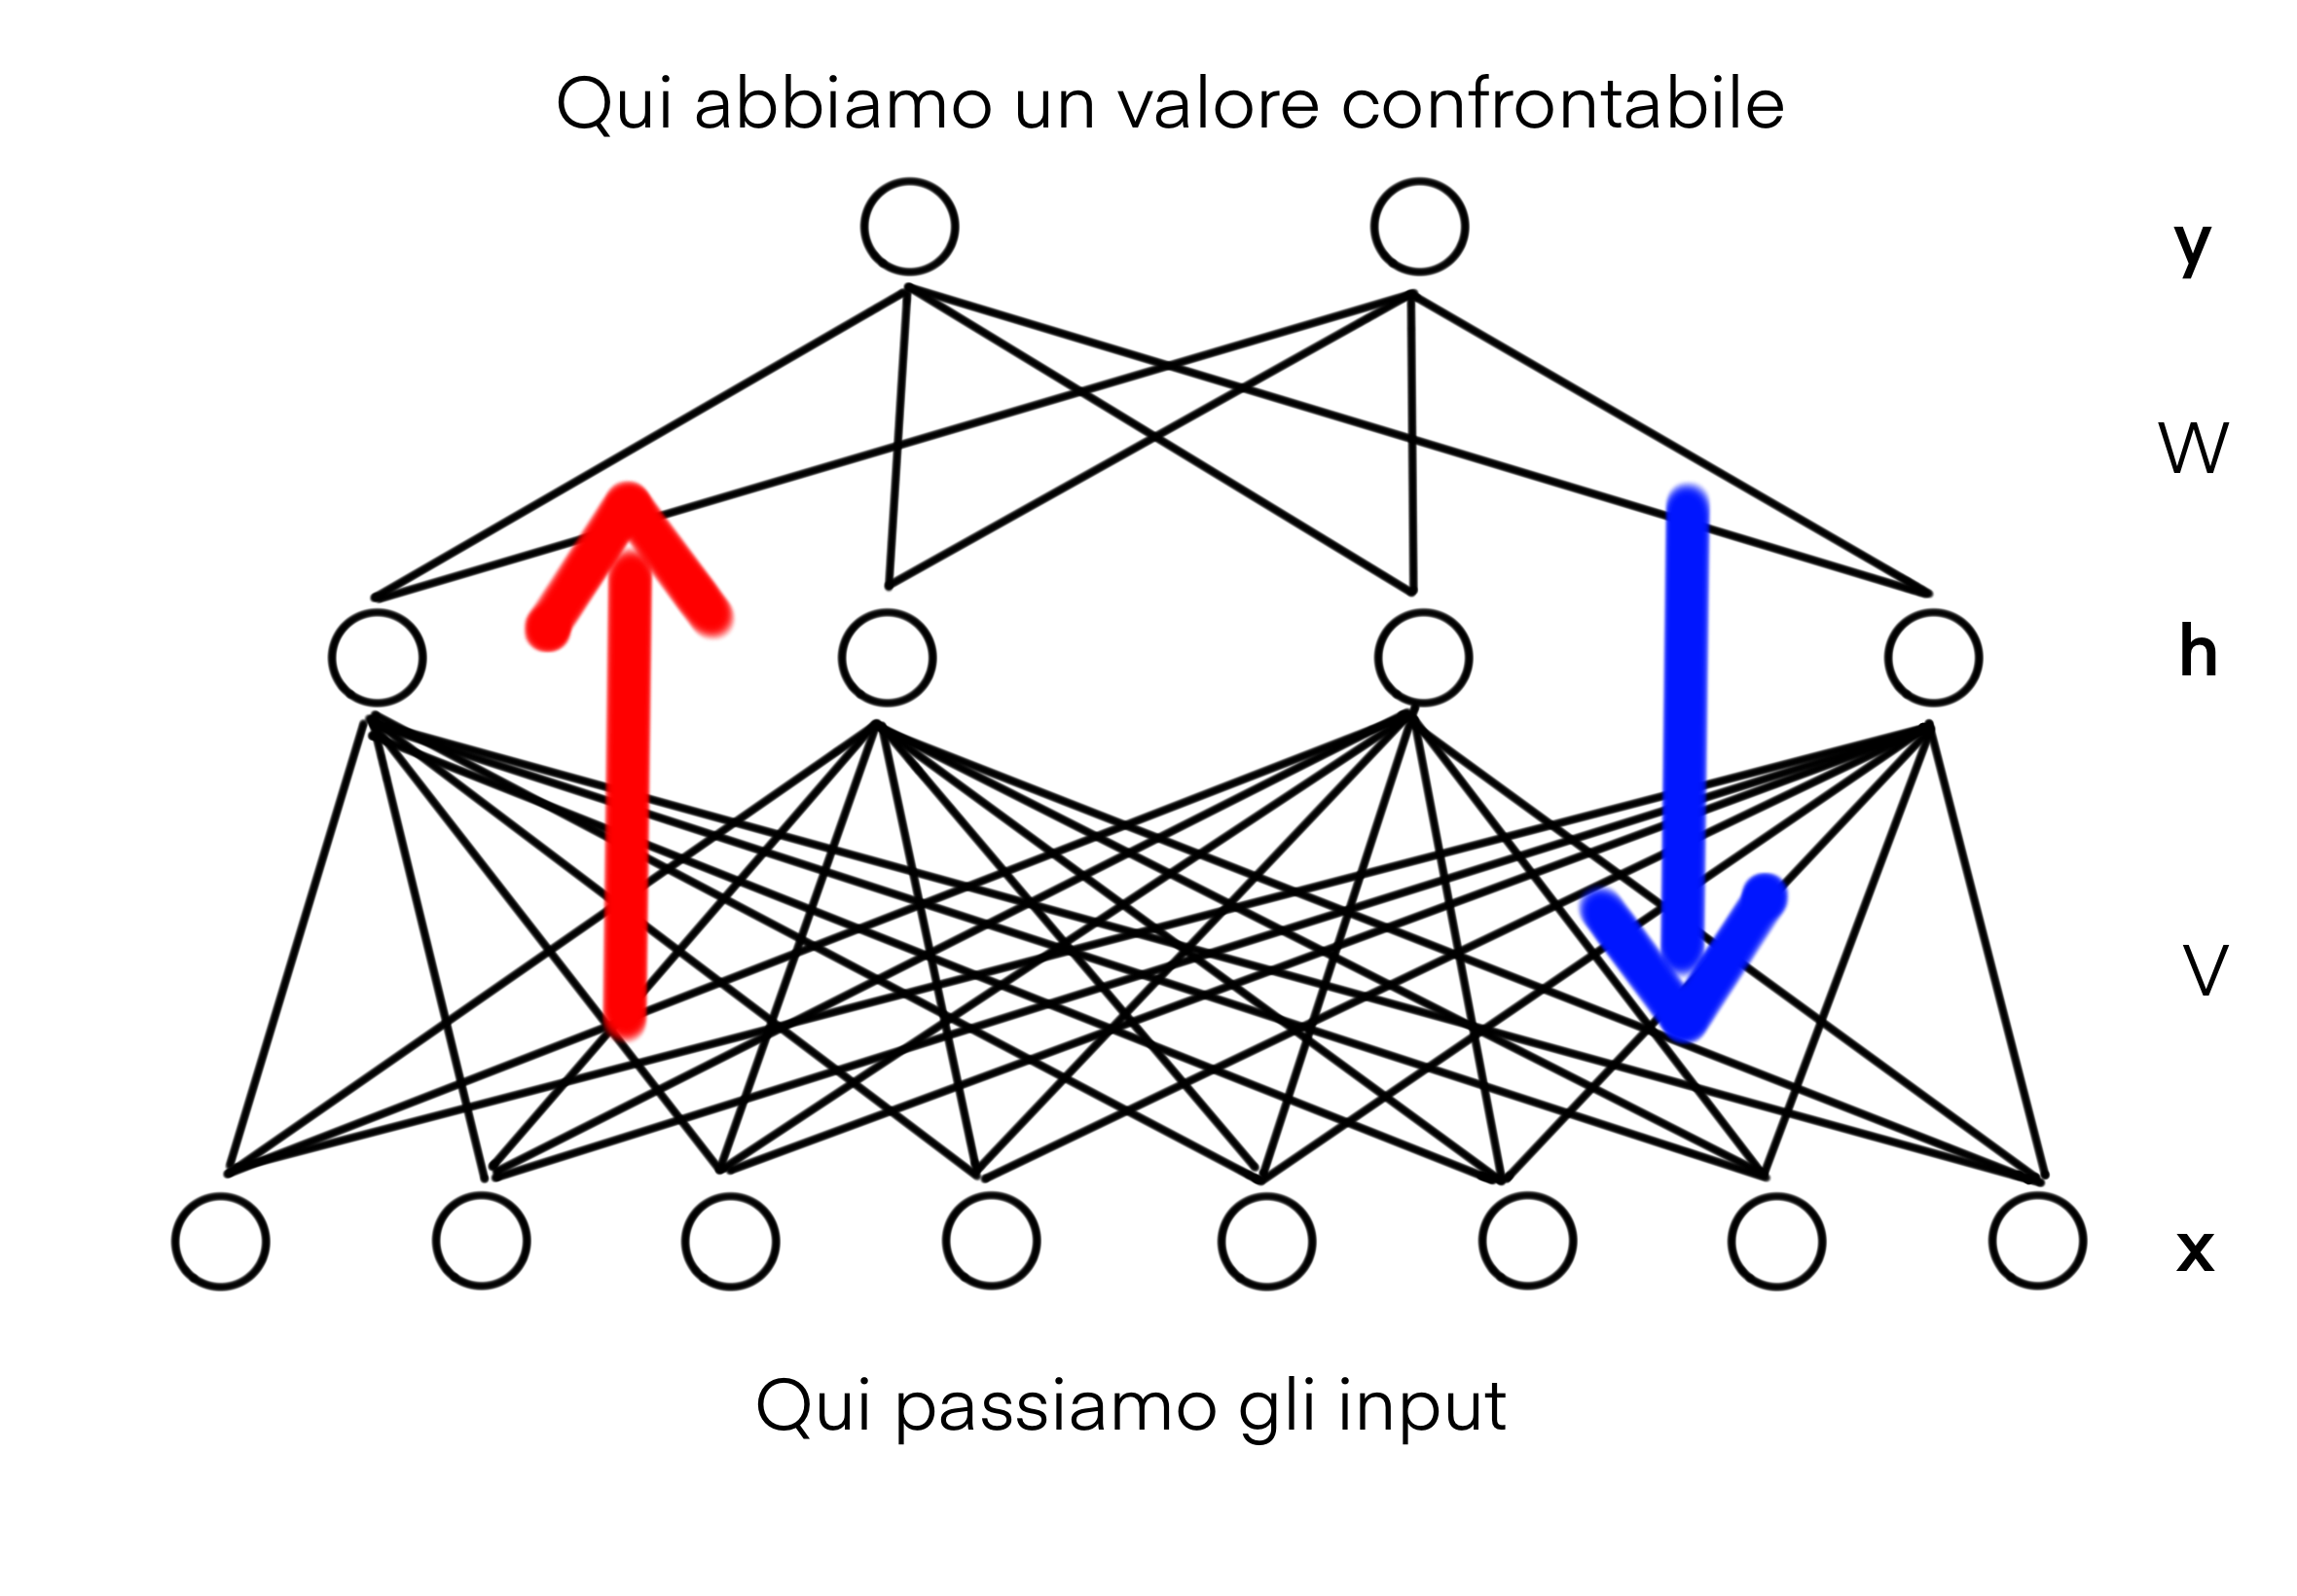
\includegraphics[width=0.5\textwidth]{backpropagation}
	\caption{Algoritmo di back-propagation, la freccia rossa indica il flusso
		del calcolo della previsione, mentre la freccia blu indica il flusso del
		calcolo dell'errore.}
	\label{fig:backpropagation}
\end{figure}

Consideriamo una rete feedfoward a due strati di connessioni con unità di input
$x_k$, unità interne $h_j$ e unità di output $y_i$. Indichiamo con $t^\mu_i$ il
valore della risposta correttà per ogni unità di output $i$ sull'input $\mu$.\\
Nell'esempio in questione, dunque abbiamo due strati di connessioni che devono
essere aggiornati. Spieghiamo i passi dell'algoritmo:

\begin{enumerate}
	\item \textbf{Input}: abbiamo in input un pattern d'ingresso $x$;

	\item \textbf{Forward pass 1}: calcoliamo l'attivazione di tutte le unità
	      interne $h_j = \phi(\sum_{k} v_{jk} x_k)$, dove $v_{jk}$ è il
	      peso della connessione tra l'unità in input $k$ e l'unità interna $j$;

	\item \textbf{Forward pass 2}: calcoliamo l'attivazione di tutte le unità di
	      output $y_i = \phi(\sum_{j} w_{ij} h_j)$, dove $w_{ij}$ è il peso
	      della connessione tra l'unità interna $j$ e l'unità di output $i$;

	\item \textbf{Calcolo dell'errore 1}: ora vogliamo minimizzare l'errore, quindi
	      confrontiamo il risultato ottenuto con il risultato corretto. Calcoliamo
	      la correzione dei pesi sinaptici come
	      \begin{equation*}
		      \Delta w_{ij} = \eta (t_i - y_i) \phi'(A_i) h_j,
	      \end{equation*}
	      dove $\eta$ è il tasso di apprendimento, $t_i$ è il
	      valore corretto dell'unità di output $i$, $y_i$ è il valore ottenuto
	      dall'unità di output $i$, $\phi'(A_i)$ è la derivata della funzione di
	      attivazione dell'unità di output $i$ e $h_j$ è l'attivazione dell'unità
	      interna $j$. Infatti, abbiamo applicato la regola delta;

	\item \textbf{Calcolo dell'errore 2}: calcoliamo l'errore dell'unità interna
	      $j$ come:
	      \begin{equation}
		      \Delta v_{jk} = - \eta \frac{\partial E}{\partial v_{jk}}
	      \end{equation}
	      ovvero, calcoliamo l'errore dell'unità interna $j$ come la somma degli
	      errori delle unità di output $i$ moltiplicati per i pesi delle
	      connessioni tra l'unità interna $j$ e l'unità di output $i$.
	      Calcoliamo le derivate:

	      \begin{equation}
		      \Delta v_{jk} = \eta \sum_{i} (t_i - y_i) \phi'(A_i) w_{ij} \phi'(A_j) x_k
	      \end{equation}
\end{enumerate}

Dunque, l'algoritmo di back-propagation si svolge in due fasi: nella prima fase
sono calcolati i valori di attivazione di ciascuno strato in ordine. In questo
modo viene calcolata la previsione della rete. Nella seconda fase, invece, sono
modificati i pesi per ridurre l'errore. Poiché le unità di output forniscono un
risultato direttamente confrontabile con il risultato corretto, viene applicata
la regola delta. In questo modo, viene calcolato l'errore commesso da ciacuna
unità di output. Questo errore, passa allo strato inferiore seguendo i pesi
sinaptici di ciascuna connessione, in questo modo viene calcolato l'errore per
ciascuna unità sottostante. Dunque sono modificati i pesi sinaptici e di nuovo
viene calcolato l'errore per lo strato inferiore. Fino ad arrivare allo strato
di input.
Riporto la formula per il calcolo della correzione dei pesi sinaptici per le
unità di output:

\begin{equation*}
	\Delta w_{ij} = \eta (t_i - y_i) \phi'(A_i) h_j
\end{equation*}

E la formula per il calcolo dell'errore per le unità interne:

\begin{equation*}
	\Delta v_{jk} = \eta \sum_{i} (t_i - y_i) \phi'(A_i) w_{ij} \phi'(A_j) x_k
\end{equation*}

Notiamo la similitudine tra le due formule: se consideriamo l'errore
come $E = (t_i - y_i) \phi'(A_i)$, per le unità di output, e l'errore come
$E = \sum_{i} (t_i - y_i) \phi'(A_i) w_{ij} \phi'(A_j)$, per le unità interne,
possiamo scrivere le formule in modo più compatto:

\begin{equation*}
	\Delta w_{ij} = \eta E_j x_j
\end{equation*}

Dove $w_{ij}$ è il peso della connessione tra l'unità $j$ e l'unità $i$, $E_j$
è l'errore dell'unità $j$ e $x_j$ è l'attivazione dell'unità $j$.
Comprendiamo ora la formula per il calcolo dell'errore per le unità interne:

\begin{equation*}
	E = \sum_{i} (t_i - y_i) \phi'(A_i) w_{ij} \phi'(A_j)
\end{equation*}

abbiamo $(t_i - y_i)$ che rappresenta l'errore dell'unità di output $i$, questo
valore viene moltiplicato per la derivata della funzione di attivazione, in
questo modo otteniamo l'errore dell'unità di output $i$. A questo errore
moltiplichiamo il peso della connessione tra l'unità interna $j$ e l'unità di
output $i$. Infatti, il peso della connessione indica quanto l'unità interna
$j$ contribuisce al valore dell'attivazione dell'unità di output $i$ e dunque
quanto influisce sull'errore dell'unità di output $i$. A questo punto, ripetiamo
il calcolo per tutte le unità di output e sommiamo i risultati, così otteniamo
l'errore dell'unità interna $j$. Moltiplichiamo l'errore così ottenuto per la
derivata del valore di attivazione, che rappresenta l'intensità del segnale;
ovvero riduciamo l'errore se il segnale in input era molto basso e lo aumentiamo
se il segnale era molto forte. Infine, applichiamo la regola delta per calcolare
la correzione dei pesi sinaptici.
\subsection{Momentum}

Un metodo per incrementare la velocità di apprendimento riguarda l'adozione del
momentum, ovvero viene aggiunta l'inerzia allo spostamento sulla superficie
dell'errore, questo effetto si ottiene aggiungendo al calcolo della modifica di
ciascuna connessione una frazione della modifica ottenuta all'istante
precedente.

\begin{equation}
	\Delta w^t_{ij} = \eta E_i x_j + \alpha \Delta w^{t-1}_{ij}
\end{equation}

Dove $\alpha$ è la costante di momentum che contraolla la quantità di inerzia
fornita alla modifica sinaptica. Tipicamente, $\alpha$ è fissato intorno a
$0.8$.\\
La presenza del momentum favorisce l'avanzamento su superfici piatte o
semi-piatte e riduce le oscillazioni permettendo così l'adozione di valori più
elevati per il tasso di apprendimento ($\eta$).

\subsubsection{Parametri addattivi}

Il tasso di apprendimento e la costante di momentum possono essere adattati
dinamicamente durante il processo di apprendimento, in modo da ottenere una
velocità di apprendimento ottimale, dunque la pallina si muove più velocemente o
più lentamente a seconda della superficie su cui si trova e del percorso
effettuato. Non solo anche l'accellerazione può essere adattata
dinamicamente.\\
Non solo, si può aumentare il tasso di apprendimento per i pattern che sono
sotto-rappresentati, ovvero per quei pattern che sono pochi in numero nel set di
apprendimento, ma sono ben più frequenti nel mondo reale.\\
Oppure, si utilizza un tasso di apprendimento inversamente proporzionale al
numero di connessioni per ciascun nodo. Ovvero, maggiore è il numero di
connessioni, minore è il tasso di apprendimento. Questo perché, se un nodo ha
molti input, allora il suo contributo all'errore è minore rispetto a un nodo con
pochi input.\\

\subsection{Pesi sinaptici iniziali}

I valori iniziali dei pesi sinaptici sono importanti in quanto determinano i
punto di partenza della rete neurale sulla superficie di errore. La
backpropagation richiede che i pesi sinaptici assumano valori diversi tra loro,
altrimenti tutti i pesi sinaptici si muoverebbero nella stessa direzione e con
la stessa velocità. Date le proprietà delle funzioni di attivazione,
considerando per esempio la sigmoide, oppure la tangente iperbolica, la derivata
ha valore massimo in $0$. Dunque se i pesi sinaptici sono inizializzati vicino
allo 0, per esempio nell'intervallo $[-0.5, 0.5]$, allora la derivata della
funzione di attivazione ha valore elevato e dunque la rete neurale apprende più
velocemente.\\
Si consiglia di limitare il valore dei pesi sinaptici entro $\pm 1 /
	\sqrt{k_i}$, dove $k_i$ è il numero di unità di input dell'unità $i$-esima.\\
Questa procedura stabilisce limiti diversi per i vari nodi della rete e assicura
che la somma pesata degli input per ciascun nodo sia intorno a 0. Per cui, la
funzione sigmoide e la tangente iperbolica hanno derivata massima.

\subsection{Addizione di rumore}

Un modo semplice per cercare di uscire dai minimi locali consiste nell'applicare
un po' di rumore durante l'apprendimento della rete. Ovvero, si fanno variare
i valori dei pesi sinaptici aggiungendo dei piccoli valori estratti da una
distribuzione uniforme di numeri casuali intorno allo zero. Metaforicamente, è
come introdurre dei piccoli terremoti sulla superficie dell'errore, per cercare
di forzare la pallina a uscire dai minimi locali. Se l'errore continua a calare
allora il rumore viene ridotto, altrimenti viene aumentato. Fondamentalmente si
costringe la pallina a muoversi in modo casuale sulla superficie dell'errore, se
l'errore è elevato, ma la pallina è bloccata in un minimo locale o in una
superficie piatta.


\section{Quickdrop}

Fahlman ha proposto un algoritmo di discesa del gradiente completamente locale
(per cui la modifica di una connessione richiede solo informazione direttamente
disponibile a livello dell'unità presinaptica e di quella postsinaptica). Il
metodo è basato sull'assunzione che la discesa della superficie di errore di un
singolo peso sinaptico è relativamente indipendente dalle modifiche che vengono
apportate agli altri pesi sinaptici. Questa assunzione è in realtà
un'approssimazione, tuttavia l'algoritmo che si ottiene è molto molto rapido,
per cui, nel momento in cui ci si ritrova in una stagnazione, è sufficiente far
ripartire l'algoritmo da un punto diverso.\\
Il metodo consiste nel modificare ciascun peso sinaptico in base al confronto in
due tempi successivi della variazione dell'errore ottenuta grazie a quel peso:
se la variazione è nella stessa direzione della variazione precedente, allora il
peso verrà modificato nella stessa direzione del cambiamento effettuato in
precedenza, altriemnto esso verrà modificato nella direzione opposta. Per ogni
peso della rete, la regola di modifica sinaptica è la seguente:

\begin{equation}
	\Delta w^t = \frac{S^t}{S^{t-1} - S^t}\Delta w^{t-1}
\end{equation}

Dove $S$ esprime la variazione della funzione di errore $E_W$ su tutti i pattern
di addestramento per quel peso sinaptico:

\begin{equation}
	S = \frac{\partial E_W}{\partial w}
\end{equation}

Per cui, considerato una rete come quella della back-propagation (vedi
\autoref{fig:backpropagation}), la variazione dell'errore per un peso sinaptico,
($S$) è:

\begin{equation}
	S_{ij} = - \sum_{\mu} E^\mu_i x^\mu_j
\end{equation}

Dove $S_{ij}$ è la variazione dell'errore per il peso sinaptico che connette
l'unità $j$ all'unità $i$, $E^\mu_i$ è l'errore dell'unità $i$ per il pattern
$\mu$ e $x^\mu_j$ è l'uscita dell'unità $j$ per il pattern $\mu$.\\
Dato che quando $S$ assume la stessa direzione e valore per due epoche
consecutive, il cambiamento dei pesi sinaptici cresce all'infinito, viene
applicato un limite $\lambda$: $\Delta w^t = \lambda \Delta w^{t-1}$ (di solito
$\lambda = 1.75$). Infine, viene addizionata una frazione della discesa di
gradiente per evitare il "congelamento" dei pesi.

\section{Funzioni di attivazione}

La funzione di attivazione determina il tipo di risposta che un neurone può
emettere. Di seguito sono elencati alcuni esempi di funzioni di attivazione.

\subsection{Funzione "a gradino"}

\begin{equation*}
	\phi(A) = \begin{cases}
		1 & \text{se } A \geq \theta \\
		0 & \text{se } altrimenti
	\end{cases}
\end{equation*}

Dove $\theta$ è la soglia del neurone. Ponendo $\theta = 0$ si ottiene:

\begin{center}
	\begin{tikzpicture}[scale=1.5]
		% Asse x
		\draw[->] (-2,0) -- (2,0) node[right] {$A$};
		\foreach \x in {-1, 1}
		\draw (\x,0.1) -- (\x,-0.1) node[below] {$\x$};

		% Asse y
		\draw[-] (0,0) -- (0,1) node[above] {$y$};
		\draw (0.1,1) -- (-0.1,1) node[left] {1};

		% Funzione
		\draw[domain=-2:0,thick,variable=\x,blue] plot ({\x},{0});
		\draw[domain=0:2,thick,variable=\x,blue] plot ({\x},{1});
	\end{tikzpicture}
\end{center}

Alternativamente, l'output può essere bipolare:

\begin{equation*}
	\phi(A) = \begin{cases}
		1  & \text{se } A \geq \theta \\
		-1 & \text{se } altrimenti
	\end{cases}
\end{equation*}

\subsection{Funzione lineare}

Maggiori informazioni sono trasmesse se si utilizza una funzione continua
lineare:

\begin{equation*}
	\phi(A) = kA
\end{equation*}

dove $k$ è una costante. Le funzioni continue permettono al neurone di
trasmettere una gradazione di segnali di vaira intensità che può essere
opportunamente sfruttata dai neuroni riceventi.

\begin{center}
	\begin{tikzpicture}
		\begin{axis}[
				xlabel=$A$,
				ylabel={$\phi(A)$},
				axis lines=middle,
				xtick={-1, 0, 1},
				ytick={-1, 0, 1},
				ymin=-1.5,
				ymax=1.5,
				xmin=-1.5,
				xmax=1.5,
			]

			\addplot[domain=-1:1, blue, thick] {x};
		\end{axis}
	\end{tikzpicture}
\end{center}

\subsection{Funzione sigmoide}

In alcune situazione risulta utile forzare l'output del neurone ad assumere
valori compresi in un intervallo, per esempio $[0, 1]$ o $[-1, 1]$. Infatti, in
questo modo si può interpretare l'output come una probabilità o come una
misura di confidenza. La funzione sigmoide o logistica è definita come:

\begin{equation*}
	\phi(A) = \frac{1}{1 + e^{-kA}}
\end{equation*}

Dove $k$ è la costante che controlla l'inclinazione della curva; per $k
	\rightarrow \infty$ la funzione si comporta come una funzione a gradino. Le
rette $y = 0$ e $y = 1$ sono asintoti orizzontali della funzione sigmoide.

\begin{center}
	\begin{tikzpicture}
		\begin{axis}[
				xlabel=$A$,
				ylabel={$\phi(A)$},
				axis lines=middle,
				xtick={-1, 0, 1},
				ytick={0, 0.5, 1},
				ymin=-0.5,
				ymax=1.5,
				xmin=-1.5,
				xmax=1.5,
			]

			\addplot[domain=-1.9:1.9, blue, thick] {1/(1 + exp(-2*x))};
			\addplot[domain=-1.9:1.9, black, dashed] {1};
		\end{axis}
	\end{tikzpicture}
\end{center}

Una funzione simile è la tangente iperbolica ($\tanh(kA)$) che ha le rette $y =
	-1$ e $y = 1$ come asintoti orizzontali.\\
Nella maggior parte dei modelli tutti i neuroni eccetto i neuroni di input
(recettori) utilizzano la medesima funzione di attivazione.

\subsection{Funzione a base radiale}

Una funzione a base radiale genera un output non-negativo per tutti i pattern ed
è simmetrica rispetto al baricentro di un gruppo di input. Le funzioni più
comunemente usaet sono delle variazioni della funzione gaussiana:

\begin{equation*}
	\phi(A) = \exp(-kA^2)
\end{equation*}

La cui derivata prima è esprimibile in funzione dell'output generato:

\begin{equation*}
	\frac{d\phi(A)}{dA} = -2kA\phi(A)
\end{equation*}

\begin{center}
	\begin{tikzpicture}
		\begin{axis}[
				xlabel=$A$,
				ylabel={$\phi(A)$},
				axis lines=middle,
				xtick={-1, 0, 1},
				ytick={0, 0.5, 1},
				ymin=-0.5,
				ymax=1.5,
				xmin=-1.5,
				xmax=1.5,
			]

			\addplot[domain=-1.9:1.9, blue, thick] {exp(-2*x^2)};
		\end{axis}
	\end{tikzpicture}
\end{center}

Le funzioni a base radiale sono particolarmente utili nel caso in i pattern di
input si distribuiscano in gruppetti nello spazio; in questo caso durante
l'apprendimento ciascuna unità centra la propria risposta sul baricentro di un
gruppetto di pattern.\\

Moody e Darken hanno proposto di utilizzare la seguente funzione gaussiana:

\begin{equation*}
	\phi(A)_i = \frac{\exp(\frac{(A - \mu_i)^2}{2\sigma_i^2})}%
	{\sum_{k}\exp(\frac{(A - \mu_k)^2}{2\sigma_k^2})}
\end{equation*}

Dove $\mu_i$ e $\sigma_i$ sono rispettivamente la media e la varianza della
funzione dell'unità $i$ e il denominatore è la sommatoria dell'output di tutti i
nodi $k$ dello stesso strato. Per cui il vettore di attivazione dell'intero
strato è normalizzato.

\subsection{Funzioni logaritmiche}

Per reti che possiedono un elevato numero di unità presinaptiche, è utile
impiegare funzioni che non sono sottoposte a saturazione (cioè se diventa
difficile cambiare i pesi sinaptici). In questi caso è utile utilizzare una
funzione logaritmica:

\begin{equation*}
	\phi(A) = \begin{cases}
		\log(1 + A) & \text{per } A \geq 0 \\
		\log(1 - A) & \text{per } A < 0
	\end{cases}
\end{equation*}

Che ha derivata:

\begin{equation*}
	\phi'(A) = \begin{cases}
		\frac{1}{1 + A} & \text{per } A \geq 0 \\
		\frac{1}{1 - A} & \text{per } A < 0
	\end{cases}
\end{equation*}

\begin{center}
	\begin{tikzpicture}
		\begin{axis}[
				xlabel=$A$,
				ylabel={$\phi(A)$},
				axis lines=middle,
				xtick={-10, 0, 10},
				ytick={0, 2.5, 5},
				ymin=-2.5,
				ymax=7.5,
				xmin=-15,
				xmax=15,
			]

			\addplot[domain=0:19, blue, thick] {ln(1 + x)};
			\addplot[domain=-19:0, blue, thick] {ln(1 - x)};
		\end{axis}
	\end{tikzpicture}
\end{center}



\end{document}
